\JWlone{Evaluation}
\label{sec:evaluation}

This chapter evaluates the usefulness, the accuracy and the overhead the energy
model imposes. The model's strenghts and weaknesses are pointed out and it is
compared to a simple computing time based model.


% #  ERROR OF ESTIMATION  ######################################################
\JWltwo{Error of Estimation}
\label{sec:error}

\begin{figure}
  \centering
    \includegraphics[width=\textwidth]{fig/hist-models.eps}
  \caption{Histogram of percent error, sophisticated versus simple model}
  \label{fig:err-hist}
\end{figure}

\begin{figure}
  \centering
    \includegraphics[width=\textwidth]{fig/hist-model-15W.eps}
  \caption{Histogram of percent error for \SI{15}{\watt}\textsuperscript{+}--benchmarks}
  \label{fig:err-hist-15}
\end{figure}

\begin{figure}
  \centering
    \includegraphics[width=\textwidth]{fig/Ncpu-bench-errs.eps}
  \caption{Percent error, sophisticated versus simple model}
  \label{fig:errs-ncpu}
\end{figure}

The majority of the 3000 benchmark runs mentioned in chapter
\ref{sec:benchmarks} and \ref{sec:final-model} are estimated with an error of
5\% or better as \emph{model} in figure \ref{fig:err-hist} shows. The bars named
\emph{cpu\_\-time\_\-based} are a comparison to a simple computing time based
model, discussed in a chapter of its own (\ref{sec:time-based}). The overall
worst sample was estimated with an error of about 40\% (see \emph{model} in
figure \ref{fig:errs-ncpu}). The sample is from a special benchmark run where
all four cores were enabled but mostly idle (real average power usage
\SI{8.9}{\watt}, \SI{12.5}{\watt} estimated). This erratic behavior is
explainable by the design of the model: The goal has been to develop a model
which won't produce completely faultily results but focuses on higher power
consumptions. The power consumptions observed were between \SI{6}{\watt} and
\SI{60}{\watt} and the focus has been set on the range above \SI{15}{\watt}.
This decision was motivated by the fact that a operating system will typically
spend very little time in ACPI Processor State C0 \cite{wiki:ACPI} when very
little energy is consumed. But as chapter \ref{sec:restrictions} states, the
energy model worked out in this thesis is only valid when the CPU is in state C0
all along.  Nevertheless, a similar energy model could be evolved with
particular support for low--power CPU usage and the other ACPI Processor States
in mind.

Regarding the vast majority of benchmarks---which consume more than
\SI{15}{\watt} on average---the model's estimation is clearly better. Figure
\ref{fig:err-hist-15} illustrates a percentaged error classification of the
benchmarks consuming more than \SI{15}{\watt} on average. The
\SI{15}{\watt}\textsuperscript{+}--benchmarks show an average estimation error
of only 5.3\%.


% #  COMPARISON TO SIMPLE TIME BASED MODEL  ####################################
\JWltwo{Comparison to a simple time based Model}
\label{sec:time-based}

As it is still today's standard to use computing time based models, this chapter
will compare the estimations against the more sophisticated energy model
presented here (chapter \ref{sec:final-model}).

The comparison of the overall average energy estimation error shows the benefit
of a reasonable energy model: 5.4\% versus 13.1\% for the simple computing time
based model. Figure \ref{fig:errs-ncpu} illustrates the results, where the final
energy model is listed as \emph{model} in the figures. The computing time based
model was built by only using the event \JWctr{CPU\_CLK\_UNHALTED} and is
referred to in the figures as \emph{cpu\_\-time\_\-model}. It has been fitted
using a linear regression on the same training data as the regular model,
resulting in the formula

\begin{equation}
W = 5.885J * 10^{-9} * \JWctr{CPU\_CLK\_UNHALTED}.
\end{equation}


% #  OVERHEAD IMPLEMENTATION  ##################################################
\JWltwo{Overhead of this Implementation}
\label{sec:overhead}

To evaluate the overhead of this implementation three metrics have been applied:
Running time, average power usage and unhalted CPU clock cycles. To compare the
results the \emph{473.astar} benchmark of the \JWTLspec{} benchmark suite has
been used. Besides a warm--up run every configuration has been executed ten
times. The performance events have been added consecutively in the order they
are listed in appendix \ref{appendix:chosen-events}. Before measuring the costs
of adding a counter, the system has been benchmarked without even setting up
\JWTlibpfm{} (see chapter \ref{sec:standard-software}). In the plots these
configurations are listed as \emph{0} performance events measured. Because the
unhalted CPU clock cycles are measured using the PMU (chapter {\ref{sec:pmu})
and \JWTlibpfm{} there is obviously no benchmark without even setting up
\JWTlibpfm{}.

\begin{figure}
  \centering
    \includegraphics[width=\textwidth]{fig/ctr-csts-cycles.eps}
  \caption{Counter Costs Cycles}
  \label{fig:ctr-costs-cycles}
\end{figure}

\begin{figure}
  \centering
    \includegraphics[width=\textwidth]{fig/ctr-csts-time.eps}
  \caption{Counter Costs Time}
  \label{fig:ctr-costs-time}
\end{figure}

\begin{figure}
  \centering
    \includegraphics[width=\textwidth]{fig/ctr-csts-power.eps}
  \caption{Counter Costs Power}
  \label{fig:ctr-costs-power}
\end{figure}

As one can see in figures \ref{fig:ctr-costs-cycles} and
\ref{fig:ctr-costs-time}, the number of counted performance events or using the
PMU (see chapter \ref{sec:pmu}) does not seem to correlate to the clock CPU
cycles or the time a process needs to complete. The Pearson product--moment
correlation coefficients (PCCs) \cite{wiki:PCC} are $-0.18$ with respect to the
running time and $-0.12$ to the clock cycles. Considering the average electrical
power there's some correlation (PCC: $0.72$, figure \ref{fig:ctr-costs-power}),
but the absolute value ($<$ \SI{0.3}{\watt}) is negligible.

So, this implementation does not harm the system's performance and its
contribution to the overall energy consumption is negligible.


% vim: set spell spelllang=en_us fileencoding=utf8 : syntax spell toplevel :
